\subsection{Real-Robot Implementation}~\label{exp:real_robot}
We additionally implemented the proposed framework on the tomato harvesting robot platform to verify that the planning and query pipeline can be integrated with physical sensing and execution.

The robot platform consists of a Summit mobile base equipped with a UR5e manipulator, an RGB-D camera for object perception, and a LiDAR sensor for localization. The tomato domain follows the same symbolic task model used in the controlled evaluation. The robot maintains a belief over task-relevant predicates such as tomato location, ripeness, and whether an object has already been picked or processed. Visual detections are converted into symbolic observations, and the planner selects actions such as navigation, detection, picking, scanning, placing, and discarding.

\begin{figure}[t]
    \centering
    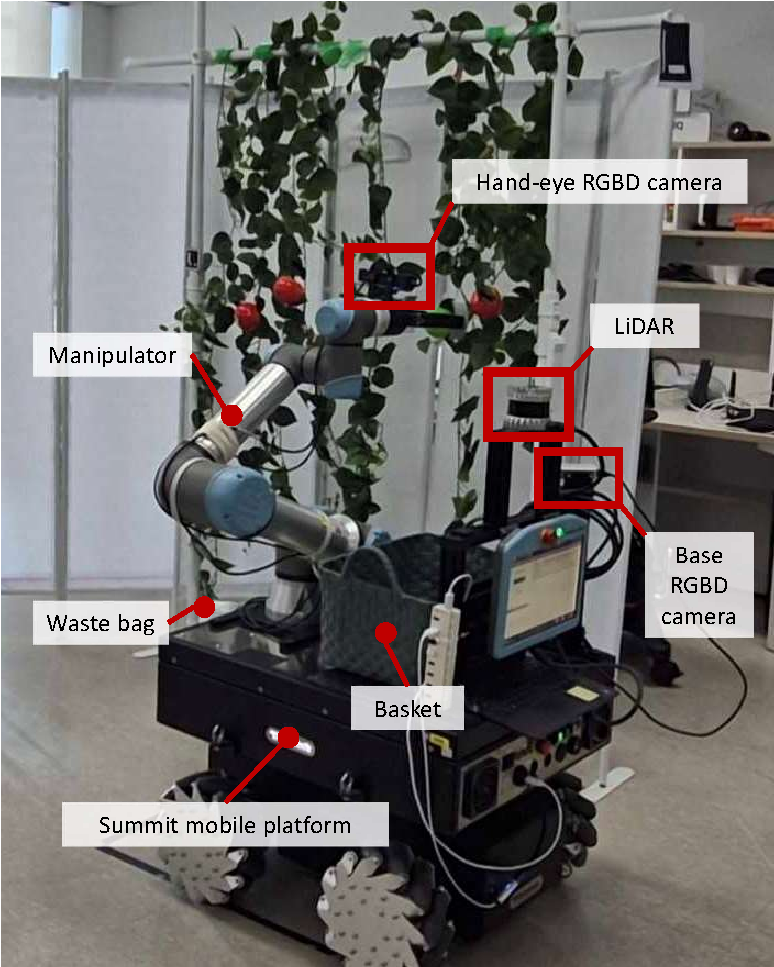
\includegraphics[width=\linewidth]{figures/real_robot/fig_robot.pdf}
    \caption{Real-robot implementation in the tomato harvesting domain.}
    \label{fig:real_robot_tomato}
\end{figure}

The implementation was conducted in a tomato harvesting environment containing multiple tomato plants and collection basket, as shown in Fig.~\ref{fig:real_robot_tomato}. The symbolic planner, belief manager, perception module, and query interface were integrated with the robot control system. Object detections obtained from the RGB-D camera were converted into symbolic predicates and provided to the planner, while navigation and manipulation commands were executed through the robot middleware.

During execution, the robot successfully performed navigation, tomato detection, harvesting, scanning, and placement behaviors while interacting with the user through the proposed query interface. User responses were incorporated into the planning process and influenced subsequent task decisions. The experiment demonstrates that the proposed framework can be deployed on a physical robot and integrated with real-world perception and execution pipelines.\footnote{Please see the supplementary video for the real-robot execution.}